% This is "sig-alternate.tex" V1.9 April 2009
% This file should be compiled with V2.4 of "sig-alternate.cls" April 2009
%
% This example file demonstrates the use of the 'sig-alternate.cls'
% V2.4 LaTeX2e document class file. It is for those submitting
% articles to ACM Conference Proceedings WHO DO NOT WISH TO
% STRICTLY ADHERE TO THE SIGS (PUBS-BOARD-ENDORSED) STYLE.
% The 'sig-alternate.cls' file will produce a similar-looking,
% albeit, 'tighter' paper resulting in, invariably, fewer pages.
%
% ----------------------------------------------------------------------------------------------------------------
% This .tex file (and associated .cls V2.4) produces:
%       1) The Permission Statement
%       2) The Conference (location) Info information
%       3) The Copyright Line with ACM data
%       4) NO page numbers
%
% as against the acm_proc_article-sp.cls file which
% DOES NOT produce 1) thru' 3) above.
%
% Using 'sig-alternate.cls' you have control, however, from within
% the source .tex file, over both the CopyrightYear
% (defaulted to 200X) and the ACM Copyright Data
% (defaulted to X-XXXXX-XX-X/XX/XX).
% e.g.
% \CopyrightYear{2007} will cause 2007 to appear in the copyright line.
% \crdata{0-12345-67-8/90/12} will cause 0-12345-67-8/90/12 to appear in the copyright line.
%
% ---------------------------------------------------------------------------------------------------------------
% This .tex source is an example which *does* use
% the .bib file (from which the .bbl file % is produced).
% REMEMBER HOWEVER: After having produced the .bbl file,
% and prior to final submission, you *NEED* to 'insert'
% your .bbl file into your source .tex file so as to provide
% ONE 'self-contained' source file.
%
% ================= IF YOU HAVE QUESTIONS =======================
% Questions regarding the SIGS styles, SIGS policies and
% procedures, Conferences etc. should be sent to
% Adrienne Griscti (griscti@acm.org)
%
% Technical questions _only_ to
% Gerald Murray (murray@hq.acm.org)
% ===============================================================
%
% For tracking purposes - this is V1.9 - April 2009

\documentclass{sig-alternate}
%\usepackage{longtable}
%\usepackage{caption}
\usepackage{graphicx}
%\usepackage{url}
%\usepackage{float}
%\usepackage{times}
%\usepackage{multirow}
%\usepackage{listings}
%\usepackage{times}
%\usepackage{paralist}
%\usepackage{epsfig}
%\usepackage{subfigure}
%\usepackage{longtable}
%%\usepackage[hypertex]{hyperref}
%\usepackage{subfigure}
\usepackage{color}
\usepackage[numbers]{natbib}
%\usepackage{ifpdf}
%\usepackage{wrapfig}
%\usepackage{float}
%\usepackage{texdraw}
%\usepackage{epsf}
%\usepackage{array}
%\usepackage{cite}
%\usepackage{enumitem}
%\usepackage{verbatim}
%\usepackage{setspace}
%\sloppy
%\usepackage{geometry}
\usepackage{listings}


\newif\ifdraft
\drafttrue
\ifdraft
\newcommand{\abhi}[1]{ {\textcolor{red} { ***Abhinav: #1 }}}
\else
\newcommand{\abhi}[1]{ {}}
\fi
\newcommand{\ty}{\texttt}


\begin{document}
%
% --- Author Metadata here ---
\conferenceinfo{XSEDE}{'13 San Diego, CA USA}
%\CopyrightYear{2007} % Allows default copyright year (20XX) to be over-ridden - IF NEED BE.
%\crdata{0-12345-67-8/90/01}  % Allows default copyright data (0-89791-88-6/97/05) to be over-ridden - IF NEED BE.
% --- End of Author Metadata ---

\title{mlRho -- The Anatomy of a Successful Campus Bridging Project}
% \titlenote{(Produces the permission block, and
%copyright information). For use with
%SIG-ALTERNATE.CLS. Supported by ACM.}}
%\subtitle{[Extended Abstract]
%\titlenote{A full version of this paper is available as
%\textit{Author's Guide to Preparing ACM SIG Proceedings Using
%\LaTeX$2_\epsilon$\ and BibTeX} at
%\texttt{www.acm.org/eaddress.htm}}}
%
% You need the command \numberofauthors to handle the 'placement
% and alignment' of the authors beneath the title.
%
% For aesthetic reasons, we recommend 'three authors at a time'
% i.e. three 'name/affiliation blocks' be placed beneath the title.
%
% NOTE: You are NOT restricted in how many 'rows' of
% "name/affiliations" may appear. We just ask that you restrict
% the number of 'columns' to three.
%
% Because of the available 'opening page real-estate'
% we ask you to refrain from putting more than six authors
% (two rows with three columns) beneath the article title.
% More than six makes the first-page appear very cluttered indeed.
%
% Use the \alignauthor commands to handle the names
% and affiliations for an 'aesthetic maximum' of six authors.
% Add names, affiliations, addresses for
% the seventh etc. author(s) as the argument for the
% \additionalauthors command.
% These 'additional authors' will be output/set for you
% without further effort on your part as the last section in
% the body of your article BEFORE References or any Appendices.

\numberofauthors{6} %  in this sample file, there are a *total*
% of EIGHT authors. SIX appear on the 'first-page' (for formatting
% reasons) and the remaining two appear in the \additionalauthors section.
%
\author{
% You can go ahead and credit any number of authors here,
% e.g. one 'row of three' or two rows (consisting of one row of three
% and a second row of one, two or three).
%
% The command \alignauthor (no curly braces needed) should
% precede each author name, affiliation/snail-mail address and
% e-mail address. Additionally, tag each line of
% affiliation/address with \affaddr, and tag the
% e-mail address with \email.
%
% 1st. author
%Scientific Applications and Performance Tuning (SciAPT),\\
%                University Information Technology Services,\\ 
%                Indiana University, Bloomington, IN, 47408\\
\alignauthor
Abhinav Thota\\
%       \affaddr{Scientific Applications and Performance Tuning (SciAPT)},\\
%       \affaddr{               University Information Technology Services,}\\
       \affaddr{              Indiana University, Bloomington, IN, 47408}\\
       \email{athota@iu.edu}
% 2nd. author
\alignauthor
Scott Michael\\
%       \affaddr{Scientific Applications and Performance Tuning (SciAPT)},\\
%       \affaddr{               University Information Technology Services,}\\
       \affaddr{              Indiana University, Bloomington, IN, 47408}\\
       \email{scamicha@iu.edu}
% 3rd. author
\alignauthor 
Sen Xu\\
%       \affaddr{Scientific Applications and Performance Tuning (SciAPT)},\\
%       \affaddr{               University Information Technology Services,}\\
       \affaddr{              Indiana University, Bloomington, IN, 47408}\\
       \email{senxu@indiana.edu}
\and  % use '\and' if you need 'another row' of author names
% 4th. author
\alignauthor 
Bernhard Haubold\\
%       \affaddr{Scientific Applications and Performance Tuning (SciAPT)},\\
%       \affaddr{               University Information Technology Services,}\\
       \affaddr{              Max-Planck Institute for Evolutionary Biology, Pl\"{o}n, Germany}\\
       \email{haubold@evolbio.mpg.de}
% 5th. author
\alignauthor 
Tom Doak\\
%       \affaddr{Scientific Applications and Performance Tuning (SciAPT)},\\
%       \affaddr{               University Information Technology Services,}\\
       \affaddr{              Indiana University, Bloomington, IN, 47408}\\
       \email{tdoak@indiana.edu}
% 6th. author
\alignauthor 
Robert Henschel\\
%       \affaddr{Scientific Applications and Performance Tuning (SciAPT)},\\
%       \affaddr{               University Information Technology Services,}\\
       \affaddr{              Indiana University, Bloomington, IN, 47408}\\
       \email{henschel@iu.edu}
}
% There's nothing stopping you putting the seventh, eighth, etc.
% author on the opening page (as the 'third row') but we ask,
% for aesthetic reasons that you place these 'additional authors'
% in the \additional authors block, viz.
% Just remember to make sure that the TOTAL number of authors
% is the number that will appear on the first page PLUS the
% number that will appear in the \additionalauthors section.

\maketitle
\begin{abstract}
Abstract ...
\end{abstract}

% A category with the (minimum) three required fields
\category{H.4}{Information Systems Applications}{Miscellaneous}
%A category including the fourth, optional field follows...
\category{D.2.8}{Software Engineering}{Metrics}[complexity measures, performance measures]

\terms{PERFORMANCE, EXPERIMENTATION}

\keywords{mlRho, high-throughput, XSEDE, BigJob, pilot-job, genetics}

\section{Introduction}
As first defined by the National Science Foundation Advisory Committee for Cyberinfrastructure's task force on
campus bridging \cite{nsf2011}, and later expanded upon by \citeauthor{stewart2012}, campus bridging is:

\begin{quotation}
``...the seamlessly integrated use of cyberinfrastructure operated by a scientist or engineer
with other cyberinfrastructure on the scientist's campus, at other campuses, and at the regional, national,
and international levels as if they were proximate to the scientist, and when working within the context of a
Virtual Organization (VO) make the 'virtual' aspect of the organization irrelevant (or helpful) to the work of
the VO. \cite{stewart2012}''
\end{quotation}

In applying this definition of campus bridging to XSEDE, one of the biggest challenges for researchers moving
from campus resources to XSEDE resources is being able to scale-up their workflows so that they are efficient
and can achieve high throughput on the larger XSEDE machines. While \citeauthor{stewart2012} identify key use
cases where campus bridging tools can improve a researcher's experience using XSEDE resources, one aspect that
is not included in their analysis is the dramatic increase in complexity that is inherent in the computational
and data storage systems when a researcher moves from his workstation to an XSEDE resource. This scale up in
complexity is in many cases a daunting prospect for a researcher new to XSEDE who may have relatively little
computational experience. Even savvy users who have experience with campus clusters can encounter issues when
scaling up to XSEDE resources.

This challenge is distinct from the challenge of providing a canonical software stack (proposed via a ROCKS
Roll by \citeauthor{stewart2012}), but can be compounded by widely divergent software environments between
campus and XSEDE resources. Even when the operating environment is not very different on XSEDE resources when
compared to campus resources researchers face problems with the sheer scale and complexity of XSEDE
resources. In our situation, campus bridging amounted to helping the researchers redesign their experiments
and scale up their workflows to move from their local workstations to IU's modest sized cluster environment,
and then on to use the much larger XSEDE machines at TACC effectively. It should be noted that, in general,
the differences in software environment between the IU campus resources and the TACC supercomputers were
superficial, the real challenge lie in dealing with scaling up the application and navigating the complexity
of a much larger system. 

In this paper we introduce a potential   In this paper we discuss how we bridged
the gap between the different approaches that are needed to succeed on machines of different sizes.

The current incarnation of the mlRho software is a serial code. However, the investigation we have conducted
with our XSEDE allocation was embarrassingly parallel in nature, so the work for each species was able to be
divided among many computational processes. To manage hundreds of processes for each of the 40+ species of
interest, we used the BigJob pilot-job tool, which is currently available on many XSEDE resources. BigJob
allowed us to distribute the analyses for each species across hundreds to a few thousand processor cores
depending on the genome sizes of species. Thus far we have conducted ML recombination rate studies on a total
of {\bf XX} individual genomes. In addition to the use of the BigJob pilot tool we have done extensive performance
analysis of the mlRho code and, with biologist and computer scientists working in conjunction, have been able
to improve the runtime of the code by a factor of {\bf XX}. We have also begun work on a parallel
implementation of the code, and will present a comparison between the parallel implementation and the BigJob
framework.

The remainder of the paper is organized as follows: section \ref{sec:background} gives some insight into the
computational methodologies and principles of biology being explored by the mlRho code. Section
\ref{sec:resources} outlines our initial estimates for the computational resources necessary to accomplish our
research agenda and the steps that were taken to secure an XSEDE allocation. In section \ref{sec:optimization}
we describe how through tracing and profiling of the code we were able to successfully optimize it and
dramatically increase its performance. Section \ref{sec:results} details the current status of the research
program and some initial science results and in section \ref{sec:conclusion} we present some conclusions.


\section{Background}\label{sec:background}
Understanding how the amazing biodiversity on our planet has arisen is a biological question that has
fascinated humans for thousands of years. It is critical to investigate the fundamental ecological and genetic
parameters (e.g., population sizes, recombination rates) to disentangle the evolutionary process of the
existing organisms. The ecological and genetic parameters play important roles in creating opportunities for
increasing genetic diversity, population divergence, and speciation. Deploying mlRho, a software package which
generates a novel measure of linkage disequilibrium, on XSEDE resources has allowed us to study these
important population-genetic parameters in a broad assembly of eukaryotic species. This approach has been
particularly fruitful when applied to the newly available genome sequences now being produced by
next-generation sequencing methods.

Although there are several methods for determining recombination rates, they can be both time and resource
intensive. We have employed a novel analytic approach that employs a new metric called the zygosity
correlation coefficient estimated using maximum likelihood (ML). This approach requires single individual
samples, but is extremely data intensive. Using the ML approach implemented in the mlRho software developed at
IU and XSEDE computational resources, we have been able to examine the recombination rates of a plethora of
species with accuracy that was previously unachievable.

\subsection{Program Description}
\texttt{mlRho} estimates mutation, recombination, and sequencing error from genome
sequences~\cite{hau10:mlr}. The underlying data consists of assembled sequencing reads obtained from a single
diploid individual. Such data are collected, for example, for the 1000 human genome project. At each sequenced
position \texttt{mlRho} reads the number of \ty{A}s, \ty{C}s, \ty{G}s, and \ty{T}s, a ``profile'', from a
file. Given a mutation and error rate, \ty{mlRho} computes two probabilities for each profile: The
probabilities of observing the profile given that the position is either mutated (heterozygous), or not
(homozygous). These probabilities depend on the mutation and error rates. By varying them, \ty{mlRho} finds
the values that maximize the overall likelihood of the data.

While mutation and sequencing error affect individual genome positions, recombination uncouples the
evolutionary history of pairs of positions. This is observable as a decorrelation of the zygosity states of
pairs of positions. To estimate recombination, \ty{mlRho} computes the probability of observing profile pairs
separated by, say, 1000 nucleotides. This is a function of the recombination rate and the single position
likelihoods.

\subsection{Linkage Disequilibrium and Recombination Rate}\label{sec:LD}
Linkage disequilibrium (LD), i.e., the non-random association of alleles at two or more loci, is an important parameter for many areas of population genetics.  In recent years, there has been a growing interest in measuring LD across a broad range of species, because a proper understanding of LD would greatly facilitate identifying the genetic loci which underlie important phenotypic variation in natural populations, as well as human diseases. More importantly, LD is a population-genetic parameter that can help ascertain recombination rate, because recombination is the primary evolutionary force that breaks down LD among genetic loci. Although a substantial body of research has been devoted to determining the evolutionary advantages of recombination~\cite{resolving-paradox}, the forces that determine recombination rates remain poorly understood. For example, we have little idea what determines the occurrence of recombination on a chromosome, what impact local DNA polymorphism has on recombination processes, and how recombination rates change over evolutionary time~\cite{stumpf}. 

Conventional approaches to measuring LD and recombination rates use population-genetic surveys. These surveys require hundreds of individuals and dozens of genetic loci. Using this method, the sampling variance associated with conventional measures of LD, such as D (a measure of LD) and $r^2$ (the square of the correlation coefficient), is huge. Due to this fact, a large number of loci are needed to obtain a reasonable estimate of LD.  Recombination rates can also be investigated by pedigree analyses and crossing experiments, but these methods cannot provide information on fine-scale recombination rates and are often difficult to perform, even in model organisms, let alone non-model species. Thus, while we know these values for a few species, there is very little comparative data to understand how these processes vary across many species.

\subsection{ A Novel Approach to Estimating LD and Recombination Rate}\label{sec:migration}

Whole genome sequences of diploid organisms include both alleles at every site of the genome (two copies of each chromosome), which can be used to determine a number of very useful population-genetic parameters in the evolution a species. With the rapid accumulation of whole genome sequences from a large number of species, a maximum likelihood (ML) approach that capitalizes on these data has recently been developed in our lab to estimate LD and examine genomic recombination patterns \cite{Lynch01112008,MEC:MEC4482}.

The general idea behind this approach is that two allelic chromosomes had a common ancestor sometime in the past (just as any two humans share a common ancestor at some point in the past), and at that time, were identical. Since that time, they have become increasingly different, due both to mutations changing their sequence, and to each chromosome recombining with other chromosomes in the population (the larger the population, the more other chromosomes there are to recombine with). If we catalog the similarities and differences between the two alleles, we can learn about this history of mutation and recombination. 

The ML approach uses this information to determine the zygosity correlation ($\Delta$) between all the pairs of sites that are separated by various distances (i.e., the probability of two sites being both homozygous or both heterozygous) in a single diploid genome, using the entire set of individual reads. Population genetic theory then links the expected value of delta to conventional measures of LD, such as D and $r^2$, suggesting that $\Delta$ can be used as a valid measure of LD on the population level.

{\center \bf Insert equation 11, 14, and 5d from Lynch unpublished.}
\begin{eqnarray}
E(\Delta) \simeq {4E(D^2)\over \pi(1-\pi)}
\label{eq:edelta}
\end{eqnarray}

 \begin{eqnarray}
E(\Delta) = {{\theta(1+\theta)(18+\rho)[A+2-22\theta \rho(3+\rho+12\theta)]} \over {(10+\rho+8\theta)A}}r^2
\label{eq:edelta}
\end{eqnarray}

 \begin{eqnarray}
A = 9+6.5\rho + 0.5\rho^2+19\theta \rho+12\theta^2\rho+\theta \rho^2+54\theta+80\theta^2+32\theta^3
\label{eq:edelta}
\end{eqnarray}


It has become clear that delta is a function of the population mutation rate ($\theta$= 4 Ne $\mu$) and population recombination rate ($\rho$ = 4Nr), from which theta and rho can be estimated.

{\center \bf Insert equation 6 and equation 5d from Lynch unpublished.}


 \begin{eqnarray}
E(\Delta) \simeq {{\theta(1+2\theta)(18+\rho)} \over {2(1+\theta)A}}
\label{eq:edelta}
\end{eqnarray}

 \begin{eqnarray}
A = 9+6.5\rho + 0.5\rho^2+19\theta \rho+12\theta^2\rho+\theta \rho^2+54\theta+80\theta^2+32\theta^3
\label{eq:edelta}
\end{eqnarray}

Thus, when rho is zero, $\Delta$ is approximated by $\theta$; when $\rho$ is infinite, $\Delta$ is approximated by u/r, a parameter that reflects the relative power of mutation versus recombination. These two parameters are critical for evaluating the mutational-hazard hypothesis for genome evolution (Lynch 2007)

Our simulation results have shown that this ML procedure generates unbiased estimates for theta and zygosity-correlation at a range of sequencing coverage (10-20x) \cite{Lynch01112008}. 
This ML technique has been fully implemented in the software package mlRho. mlRho is a highly versatile program, able to handle genomes of various sizes, and linkage analyses over hundreds of thousands of base pairs. The maximum-likelihood estimates for $\Delta$ and recombination rates are efficiently sought using the Nelder and Mead algorithm, as implemented by the GNU scientific library. Nonetheless, this analysis is computationally extremely intensive: millions to tens of billions of pairs of sites at a given distance have to be extracted from the input files (usually of giga-byte sizes) and maximum likelihood estimates of $\Delta$ have to be calculated for every distance. 

%%%%

With the rapid accumulation of whole genome sequences from a large number of species, a ML approach that capitalizes on these data has recently been developed in our lab to estimate LD and examine genomic recombination patterns~\cite{Lynch01112008,MEC:MEC4482}. Whole genome sequences of diploid organisms include both alleles at every site of the genome, and the ML approach uses this information to determine the zygosity correlation (delta) between all the pairs of sites that are at various distances (i.e., the probability of two sites being both homozygous or both heterozygous) in a single diploid genome, using the entire set of individual reads. Population genetic theory then links the expected value of delta to conventional measures of LD, D and $r^2$ (Lynch, unpublished). 
%
%%{\center \bf Insert equation 11, 14, and 5d from Lynch unpublished.}
%\begin{eqnarray}
%E(\Delta) \simeq {4E(D^2)\over \pi(1-\pi)}
%\label{eq:edelta}
%\end{eqnarray}
%
%  \begin{eqnarray}
%E(\Delta) = {{\theta(1+\theta)(18+\rho)[A+2-22\theta \rho(3+\rho+12\theta)]} \over {(10+\rho+8\theta)A}}r^2
%\label{eq:edelta}
%\end{eqnarray}
%
%  \begin{eqnarray}
%A = 9+6.5\rho + 0.5\rho^2+19\theta \rho+12\theta^2\rho+\theta \rho^2+54\theta+80\theta^2+32\theta^3
%\label{eq:edelta}
%\end{eqnarray}
%
%
%It has become clear that delta is a function of the population mutation rate (theta=4Nu) and population recombination rate ($\rho=4Nr$). 
%
%%{\center \bf Insert equation 6 and equation 5d from Lynch unpublished.}
%
%
%  \begin{eqnarray}
%E(\Delta) \simeq {{\theta(1+2\theta)(18+\rho)} \over {2(1+\theta)A}}
%\label{eq:edelta}
%\end{eqnarray}
%
%  \begin{eqnarray}
%A = 9+6.5\rho + 0.5\rho^2+19\theta \rho+12\theta^2\rho+\theta \rho^2+54\theta+80\theta^2+32\theta^3
%\label{eq:edelta}
%\end{eqnarray}
%
%\abhi{explain equations?} \\
%\abhi{get figure 1}
%
%
%Thus, when rho is zero, delta is approximated by theta; when rho is infinite, delta is approximated by u/r, a parameter that reflects the relative power of mutation versus recombination. These two parameters are critical for evaluating the mutational-hazard hypothesis for genome evolution~\cite{lynch-origins}.
%
%Previous simulation results have shown that this ML procedure generates unbiased estimates for theta and zygosity-correlation at a sequencing coverage of 18-20x {\bf(Figure 1)}. More importantly, a correction technique that can eliminate the bias for these parameters at low coverage (e.g., 8x coverage, the typical coverage of most available genomes) has been developed in our lab {\bf (Figure 1)}. 
%
%{\center \bf Insert figures here.}
%
%
%This ML technique has been fully implemented in the software package mlRho. mlRho is a highly versatile program, able to handle genomes of various sizes, and linkage analyses over hundreds of thousands of base pairs. The maximum-likelihood estimates for theta, delta, and rho are efficiently sought using the Nelder and Mead algorithm, as implemented by the GNU scientific library. Nonetheless, this analysis is computationally extremely intensive: millions to tens of billions of pairs of sites at a given distance have to be extracted from the input files (usually of giga-byte sizes) and maximum likelihood estimates of delta have to be calculated for every distance. 
%
%%%%

\section{Deploying mlRho on XSEDE \\Resources}\label{sec:resources}
We have been using Quarry, a local IU resource before we decided to use XSEDE resources. Quarry is a 2960 core machine, where as Ranger is 	a 62,976 core machine, Kraken is a 112,896 core machine and Stampede is a 102400 core machine. \abhi{comment to self, consider adding a table}  The environment on Quarry is similar to that of XSEDE machines referred to here and the way users access it are also similar. The central difference is the size of the machines and therefore the biggest challenge is scaling our workflow accordingly. We explain how we made the transition and discuss the tools that we used to succeed on XSEDE.
\begin{table}
\centering
\begin{tabular}{| l  | l  | l  | l  | l  | l  | l  |} \hline
	&Quarry & Ranger & Stampede & Kraken\\ \hline
Nodes & 370 & 3936 & 6400 & 9408   \\ \hline
\# Cores	& 2960  & 62976&102400 & 112896\\ 
\hline

\end{tabular}
\caption{\abhi{decide table vs plot}  } 
\label{table:cache_comp}
\end{table}


\begin{figure} %[h!] % t=top, b=bottom, h=here, p=separate page
\centering
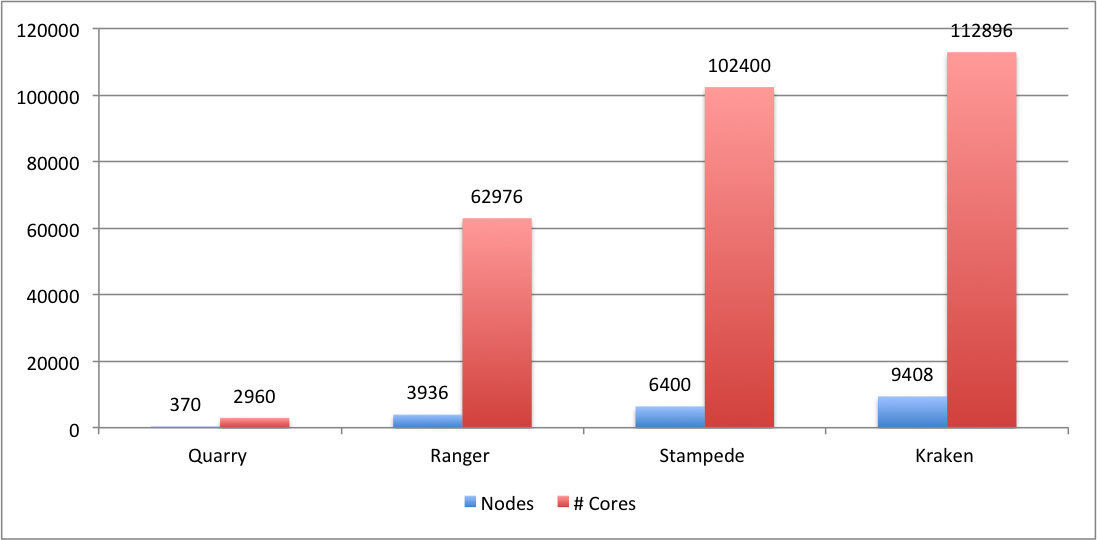
\includegraphics[width=0.48\textwidth]{figures/cores-nodes.png}
\caption{\abhi{replace with gnuplot version}}
\label{fig:scaling}
\end{figure}

\subsection{Transition to XSEDE}
\abhi{notes: startup alloc help -- CBridgers's help needed, scalability tests, etc}
We were faced with multiple questions at the start. Which of the large XSEDE machines suits us the best? Should we use more than one machine? How many SUs do we need to complete our research? Should we do everything we can or compress the amount of work we want to do depending on the number of SUs we can get from XSEDE?

We started by requesting startup allocations on Ranger and Kraken.  \abhi{cite something?} While it is possible to get good throughput submitting serial jobs to the scheduler on Quarry, this is not an optimal approach on machines like Ranger and Kraken. The scheduling policies on large machines usually favor large jobs. Many supercomputing centers have policies that limit the number of jobs a user can have in the queue. 


\subsubsection{Research Plan}\label{sec:plan}

\abhi{change the following paragraph to indicate what we actually did and why. i.e. doing more kbp/genome and may be more genomes}
We plan to use mlRho to estimate the LD and recombination patterns out to 100 kilo base-pair (kbp) distances for 46 diploid eukaryotic genomes, covering a broad range of genome sizes.%, as shown in table~\ref{table:genome_list}. 
The 100 kbp cutoff value is chosen because theory suggests that a good measure
of LD in a genome should span at least 50$-$100 kbp. Given that in eukaryotes, recombination rates range
between 0.001$-$1 event per Mbp~\cite{annurev-genom-082410-101412}, a 100 kbp window across a genome provides
a good basis for capturing the signature of crossover events that occur 1 or 2 times per chromosome arm per
meiotic event.

Our approach to linkage analyses requires diploid genomes that have not been intentionally inbred  (e.g., some plant genomes) or sequenced from several individuals. The list of 46 species are carefully selected from several important taxonomic groups to represent organisms with different ecology, population history, and reproductive strategies  (e.g., asexual vs. sexual). This list  thus constitutes a core dataset to develop a broad survey of linkage disequilibrium, population recombination rate, and population histories across eukaryotes. Furthermore, we have included genomes from multiple individuals for both {\it Daphnia pulex} and humans to explore intraspecific differences in linkage patterns and population histories. 

\subsubsection{Design of Experiments}
We have carefully constructed a detailed plan on how to proceed with our experiments. In section \ref{sec:tests}, we have shown that we can scale to 128 processes reading from the same file with no performance degradation. We estimate that we can feasibly scale-up to $\approx$500 processes reading from the same data file, without noticeable performance degradation. By making multiple copies of the data file, we could scale-up to $\approx$ 5000 processes. Job requests of 5000 processes on Ranger and Kraken are appropriate and we have not experienced extremely long wait times with past BigJob experiments. If we succeed in implementing this design, we think we can complete our analysis within four to five months from the time of the allocation award. This proposed framework is already working on Ranger, and we are in the process of implementing it on Kraken. 

In our initial testing of the three sample genomes, we worked out a few issues that could have affected
scalability. One of those issues was data access and file striping. When we had scaled up to 128 cores we
noticed intermittent I/O issues. Since all the concurrent instances read from a single file, if that file is
singly striped in a Lustre file system it will introduce a large load on the Lustre servers. We have remedied
this issue by moving the data files to the scratch file system on Ranger and striping the data files 16
ways. While this only occurred with the larger (11 and 31 GB) data files, we are aware that this might limit
our scalability. In the future, if I/O becomes an issue for scalability, we plan to use multiple copies of the
same data file to prevent an excessive number of concurrent processes from reading from the same file at the same time.

\subsubsection{SAGA BigJob framework}
\label{sec:bigjob}

BigJob is pilot-job tool available on many XSEDE resources such as Kraken, Ranger and Lonestar. Many researchers have successfully used BigJob~\cite{bigjob_web} to bundle hundreds of smaller jobs into larger, more manageable groups of jobs~\cite{Luckow:2008fp, async_repex11}. 

BigJob allows the user to maintain a list of processors allocated after the job request becomes active. The user can then assign these processors and start and manage jobs. For more details on the BigJob implementation see reference~\cite{saga_bigjob_condor_cloud}. The main benefit of doing this is that instead of submitting thousands of single core job requests to the queue, we can submit hundreds of large job requests ($\approx$ 500 to 5000 cores) to the queue. This reduces the overall job submissions to the queue and thereby, to an extent, time spent waiting in the queue. This job size is also more appropriate for many of the XSEDE machines. 

We plan to use BigJob to bundle our single-core serial mlRho simulations. We have integrated mlRho with BigJob and conducted several experiments on Ranger which have shown good performance and scalability. The experiments are explained in the next section. 


\subsubsection{mlRho Scalability Tests using BigJob on Ranger }
\label{sec:tests}


While each mlRho simulation is a serial job, we bundled many mlRho simulations using BigJob on Ranger. 
We used the BigJob installation already in place on Ranger. The major focus of our tests was to find out how mlRho scales when we increase the number of concurrent mlRho processes. 

We took three different organisms based on the size of their genome. We selected three sizes -- small (0.72 GB), medium (11 GB) and large (31 GB). We ran the mlRho program with each of these genomes. We started with 16 concurrent mlRho instances which are reading from the same data file, and let it run for 24 hours. We repeated this for each of these genomes with 16, 32, 64 and 128 concurrent instances. The results are shown in table~\ref{table:bj_runs} and figure~\ref{fig:scaling}.
Figure~\ref{fig:scaling} shows that the distance traveled, irrespective of the genome, size and the number of concurrent instances, increases linearly with number of concurrent instances being run. Table~\ref{table:bj_runs} shows the distance traveled by each instance in 24 hours for different genomes. This also shows that the distance traveled is a function of the size of the genome data file. As the reader can observe, distance traveled is directly proportional to the size of the genome data file. We were able to estimate the SUs required per distance per GB of genome data file using each of the three genomes -- all three estimates are nearly identical. Based on these results, we are confident that we can scale up to more than 1000 concurrent instances per genome using BigJob.




\section{Optimization and Performance Tuning of mlRho}\label{sec:optimization}
\subsection{Performance Analysis}\label{subsec:analysis}
%\subsection{Source-code Development and Optimization}
The mlRho application was developed through a collaboration of the Michael Lynch lab (at IU) and the Bernhard
Haubold lab (at the Max Planck Institute for Evolutionary Biology, Germany). This application is an implementation of
the novel ML approach. Researchers within the Research Technologies division of IU have been working together
with the mlRho application developers at IU and the Max Planck Institute for Evolutionary Biology to improve
the serial performance of the code. Since the ML approach is embarrassingly parallel, and the BigJob tool can
effectively distribute the workload to thousands of cores, research into parallelism for the code is not a priority right now. As a result of the initial investigations within Research Technologies, a new version has been recently released. 

The preliminary studies of Research Technologies has shown that further investigation into the serial
performance of the mlRho code is warranted. Particularly in the areas of I/O, memory usage, and call stack
depth. Research Technologies is planning to do a complete performance analysis of the code using Vampir to
find and remedy any of these inefficiencies in the code. 


\section{Speeding up \ty{mlRho}}
Starting with version 1.10, we looked at two aspects of \ty{mlRho} to
increase its efficiency: data handling and repeated
computation. As to data handling, many profiles occur repeatedly in a
data set and BH wrote the program \ty{formatPro} for compressing the raw
profiles. \ty{formatPro} reads profiles either from a text file, or from a BAM
file. BAM is the standard format for distributing genome alignment
files over the net~\citep{li09:seq}. \ty{mlRho} comes with documentation and example
scripts for accessing such data.

\ty{formatPro} writes a binary table of unique
profiles:
\begin{lstlisting}
/* write tag for recognizing file type */
fwrite("sum",sizeof(char),3,profileF);
/* note the number of profiles */
fwrite(&numNode,sizeof(int),1,profileF);
/* write the profiles */
fwrite(profiles,sizeof(Profile),numNode,profileF);
\end{lstlisting}
where a profile is
\begin{lstlisting}
typedef struct profile{  
  int profile[4];        /* profile               */
  int n;                 /* number of occurrences */
}Profile;
\end{lstlisting}
This binary file can be inspected using the program \ty{inspectPro}:
\begin{verbatim}
inspectPro profileDb.sum | head -n 3
#ID	Count	A	C	G	T
0	1411292	0	0	4	0
1	1410182	4	0	0	0
\end{verbatim}
In addition to the profiles file, \ty{formatPro} writes a binary file
listing the profile ID at every genome position:
\begin{verbatim}
inspectPro profileDb.pos | head -n 3
#Pos	Pro
1	0
2	1
\end{verbatim}
Finally, \ty{formatPro} writes a binary file of the contig lengths
\begin{verbatim}
inspectPro profileDb.con | head -n 3
#ID	Length
0	434
1	32
\end{verbatim}

\ty{mlRho} reads the profiles from the \ty{*.sum} file:
\begin{lstlisting}
/* read first three characters */
fread(&tag,sizeof(char),3,fp);
/* read the number of profiles */
fread(&numProfiles,sizeof(int),1,fp);
/* allocate space for profiles */
profiles = (Profile *)malloc(numProfiles*sizeof(Profile));
/* read profiles */
for(i=0;i<numProfiles;i++)
  fread(&profiles[i],sop,1,fp);
/* make profiles available for further computations */
setProfiles(profiles);
setNumProfiles(numProfiles);
\end{lstlisting}
Notice that the profiles are read individually rather than in a single
step, because we found that this was
faster. 

In the original version, the likelihood computation iterated over all
positions. Now it iterates over the much smaller number of unique profiles:
\begin{lstlisting}
for(i=0;i<numProfiles;i++){
  /* likelihood given that position is homozygous */
  lOneLoc = lOne(coverages[i],profiles[i].profile,ee);
  /* likelihood given that position is heterozygous */
  lTwoLoc = lTwo(coverages[i],profiles[i].profile,ee);
  l = lOneLoc * (1.0 - pi) + lTwoLoc * pi;
  likelihood += log(l) * profiles[i].n;
}
\end{lstlisting}
These likelihoods can be written to disk for future reference:
\begin{lstlisting}
/* write tag for identifying file */
fwrite("lik",sizeof(char),3,fp);
/* write size of data structure */
fwrite(result,sizeof(Result),1,fp);
/* save number of profiles considered */
np = getNumProfiles();
fwrite(&np,sizeof(double),1,fp);
/* write likelihoods given homozygosity */
fwrite(getLones(),sizeof(double),getNumProfiles(),fp);
/* write likelihoods given heterozygosity */
fwrite(getLtwos(),sizeof(double),getNumProfiles(),fp);
\end{lstlisting}

In the disequilibrium analysis of the original version, the
single-site likelihoods were recomputed at every step. Now they are
either read from disk or stored after the first pass across the
data. In addition, we noticed that by ignoring the order of two
profiles, we could halve the number of distinct profile pairs stored in
a search tree. The likelihood computation during traversal of this tree is now based entirely on
precomputed probabilities:
\begin{lstlisting}
void traverse(int a, Node *np, double h0, double h2, double complementHalf){
  if(np != NULL){
    traverse(a,np->left,h0,h2,complementHalf);

    b = np->key;
    li = h0*lOnes[a]*lOnes[b]
       + h2*lTwos[a]*lTwos[b]
       + complementHalf*(lOnes[a]*lTwos[b]+lTwos[a]*lOnes[b]);
    likelihood += log(li) * np->n;

    traverse(a,np->right,h0,h2,complementHalf);
  }
}
\end{lstlisting}
where \ty{h0} is the probability of observing a homozygous pair and
\ty{h2} the probability of observing a heterozygous pair. These two
quantities are a function of the rate of recombination. The variable
\ty{complementHalf} simply stores $1-(\ty{h0} + \ty{h2})$.

The combination of better data handling and careful avoidance of
repeated computation, lead to a 60-fold speedup of \ty{mlRho} while
maintaining its minimal memory requirement.
\begin{table}
\centering
\begin{tabular}{| l  | l  | l  | l  | l  | l  | l  |} \hline
	&Ranger & \multicolumn{3}{|c|}{Mason}\\ \hline
	& 1.11  & 1.10&1.11 & 1.14\\ \hline
GNU & 450 & 508 & 414 & 394   \\
\hline
Intel & 405 & 388 & 364 & 346\\
\hline
PGI &418 & N/A   & N/A &N/A\\
\hline

\end{tabular}
\caption{\abhi{placeholder}The table shoes mlRho runtimes on different machines with different compilers. The runtimes are in seconds. Compiling with the Intel compiler gave us a 10\% speedup compared to GNU/PGI compilers on Mason and Ranger. Future work could include building GSL with Intel compilers.   } 
\label{table:cache_comp}
\end{table}

\section{Validation}
To determine the accuracy of the revamped \ty{mlRho}, we simulated
sequencing data with known mutation and recombination
rates. Figure~\ref{fig:test}A shows that the mutation rate is
accurately estimated even if exceeded by the error
rate. Similarly, Figure~\ref{fig:test}B shows that the recombination rate is
slightly underestimated if the mutation rate $\theta=10^{-2}$ and
$\rho=10^{-2}$ or $\rho=10^{-3}$. However, the combination of low
mutation and recombination ($\theta=\rho=10^{-3}$) gives very noisy
results, demonstrating the method's limit of resolution.

\begin{figure}
  \begin{center}
    \resizebox{\textwidth}{!}{
      \begin{tabular}{cc}
        \textbf{A} & \textbf{B}\\
        % GNUPLOT: LaTeX picture with Postscript
\begingroup
  \makeatletter
  \providecommand\color[2][]{%
    \GenericError{(gnuplot) \space\space\space\@spaces}{%
      Package color not loaded in conjunction with
      terminal option `colourtext'%
    }{See the gnuplot documentation for explanation.%
    }{Either use 'blacktext' in gnuplot or load the package
      color.sty in LaTeX.}%
    \renewcommand\color[2][]{}%
  }%
  \providecommand\includegraphics[2][]{%
    \GenericError{(gnuplot) \space\space\space\@spaces}{%
      Package graphicx or graphics not loaded%
    }{See the gnuplot documentation for explanation.%
    }{The gnuplot epslatex terminal needs graphicx.sty or graphics.sty.}%
    \renewcommand\includegraphics[2][]{}%
  }%
  \providecommand\rotatebox[2]{#2}%
  \@ifundefined{ifGPcolor}{%
    \newif\ifGPcolor
    \GPcolorfalse
  }{}%
  \@ifundefined{ifGPblacktext}{%
    \newif\ifGPblacktext
    \GPblacktexttrue
  }{}%
  % define a \g@addto@macro without @ in the name:
  \let\gplgaddtomacro\g@addto@macro
  % define empty templates for all commands taking text:
  \gdef\gplbacktext{}%
  \gdef\gplfronttext{}%
  \makeatother
  \ifGPblacktext
    % no textcolor at all
    \def\colorrgb#1{}%
    \def\colorgray#1{}%
  \else
    % gray or color?
    \ifGPcolor
      \def\colorrgb#1{\color[rgb]{#1}}%
      \def\colorgray#1{\color[gray]{#1}}%
      \expandafter\def\csname LTw\endcsname{\color{white}}%
      \expandafter\def\csname LTb\endcsname{\color{black}}%
      \expandafter\def\csname LTa\endcsname{\color{black}}%
      \expandafter\def\csname LT0\endcsname{\color[rgb]{1,0,0}}%
      \expandafter\def\csname LT1\endcsname{\color[rgb]{0,1,0}}%
      \expandafter\def\csname LT2\endcsname{\color[rgb]{0,0,1}}%
      \expandafter\def\csname LT3\endcsname{\color[rgb]{1,0,1}}%
      \expandafter\def\csname LT4\endcsname{\color[rgb]{0,1,1}}%
      \expandafter\def\csname LT5\endcsname{\color[rgb]{1,1,0}}%
      \expandafter\def\csname LT6\endcsname{\color[rgb]{0,0,0}}%
      \expandafter\def\csname LT7\endcsname{\color[rgb]{1,0.3,0}}%
      \expandafter\def\csname LT8\endcsname{\color[rgb]{0.5,0.5,0.5}}%
    \else
      % gray
      \def\colorrgb#1{\color{black}}%
      \def\colorgray#1{\color[gray]{#1}}%
      \expandafter\def\csname LTw\endcsname{\color{white}}%
      \expandafter\def\csname LTb\endcsname{\color{black}}%
      \expandafter\def\csname LTa\endcsname{\color{black}}%
      \expandafter\def\csname LT0\endcsname{\color{black}}%
      \expandafter\def\csname LT1\endcsname{\color{black}}%
      \expandafter\def\csname LT2\endcsname{\color{black}}%
      \expandafter\def\csname LT3\endcsname{\color{black}}%
      \expandafter\def\csname LT4\endcsname{\color{black}}%
      \expandafter\def\csname LT5\endcsname{\color{black}}%
      \expandafter\def\csname LT6\endcsname{\color{black}}%
      \expandafter\def\csname LT7\endcsname{\color{black}}%
      \expandafter\def\csname LT8\endcsname{\color{black}}%
    \fi
  \fi
  \setlength{\unitlength}{0.0500bp}%
  \begin{picture}(7200.00,6720.00)%
    \gplgaddtomacro\gplbacktext{%
      \csname LTb\endcsname%
      \put(1078,704){\makebox(0,0)[r]{\strut{}$0$}}%
      \put(1078,2142){\makebox(0,0)[r]{\strut{}$0.005$}}%
      \put(1078,3580){\makebox(0,0)[r]{\strut{}$0.01$}}%
      \put(1078,5017){\makebox(0,0)[r]{\strut{}$0.015$}}%
      \put(1078,6455){\makebox(0,0)[r]{\strut{}$0.02$}}%
      \put(1210,484){\makebox(0,0){\strut{}$0$}}%
      \put(1909,484){\makebox(0,0){\strut{}$0.0002$}}%
      \put(2608,484){\makebox(0,0){\strut{}$0.0004$}}%
      \put(3307,484){\makebox(0,0){\strut{}$0.0006$}}%
      \put(4007,484){\makebox(0,0){\strut{}$0.0008$}}%
      \put(4706,484){\makebox(0,0){\strut{}$0.001$}}%
      \put(5405,484){\makebox(0,0){\strut{}$0.0012$}}%
      \put(6104,484){\makebox(0,0){\strut{}$0.0014$}}%
      \put(6803,484){\makebox(0,0){\strut{}$0.0016$}}%
      \put(176,3579){\rotatebox{-270}{\makebox(0,0){\strut{}$\hat\theta$}}}%
      \put(4006,154){\makebox(0,0){\strut{}$\epsilon$}}%
    }%
    \gplgaddtomacro\gplfronttext{%
      \csname LTb\endcsname%
      \put(5816,6282){\makebox(0,0)[r]{\strut{}simulated}}%
      \csname LTb\endcsname%
      \put(5816,6062){\makebox(0,0)[r]{\strut{}expected}}%
      \csname LTb\endcsname%
      \put(5816,5842){\makebox(0,0)[r]{\strut{}simulated}}%
      \csname LTb\endcsname%
      \put(5816,5622){\makebox(0,0)[r]{\strut{}expected}}%
      \csname LTb\endcsname%
      \put(5816,5402){\makebox(0,0)[r]{\strut{}simulated}}%
      \csname LTb\endcsname%
      \put(5816,5182){\makebox(0,0)[r]{\strut{}expected}}%
    }%
    \gplbacktext
    \put(0,0){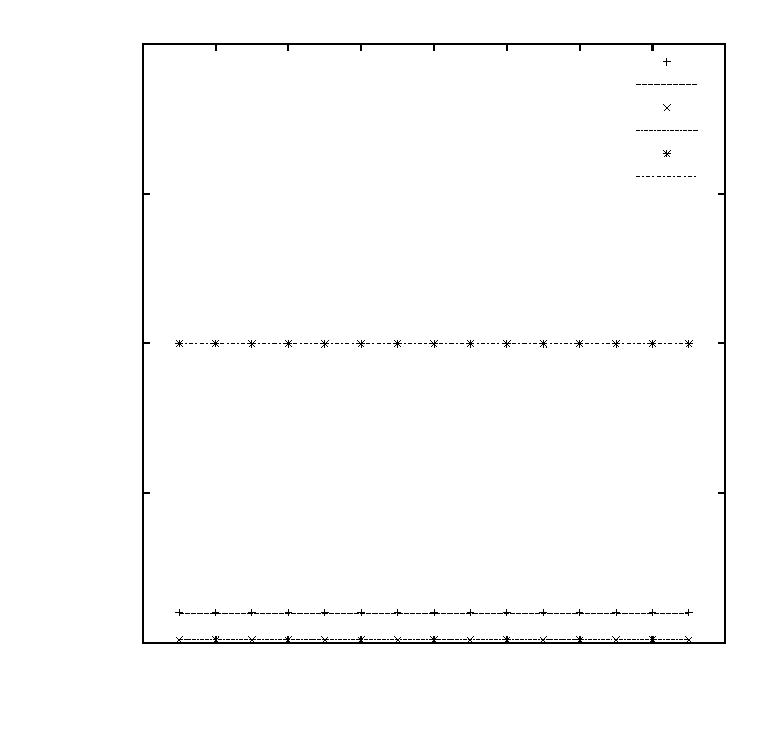
\includegraphics{figures/theta}}%
    \gplfronttext
  \end{picture}%
\endgroup
 & % GNUPLOT: LaTeX picture with Postscript
\begingroup
  \makeatletter
  \providecommand\color[2][]{%
    \GenericError{(gnuplot) \space\space\space\@spaces}{%
      Package color not loaded in conjunction with
      terminal option `colourtext'%
    }{See the gnuplot documentation for explanation.%
    }{Either use 'blacktext' in gnuplot or load the package
      color.sty in LaTeX.}%
    \renewcommand\color[2][]{}%
  }%
  \providecommand\includegraphics[2][]{%
    \GenericError{(gnuplot) \space\space\space\@spaces}{%
      Package graphicx or graphics not loaded%
    }{See the gnuplot documentation for explanation.%
    }{The gnuplot epslatex terminal needs graphicx.sty or graphics.sty.}%
    \renewcommand\includegraphics[2][]{}%
  }%
  \providecommand\rotatebox[2]{#2}%
  \@ifundefined{ifGPcolor}{%
    \newif\ifGPcolor
    \GPcolorfalse
  }{}%
  \@ifundefined{ifGPblacktext}{%
    \newif\ifGPblacktext
    \GPblacktexttrue
  }{}%
  % define a \g@addto@macro without @ in the name:
  \let\gplgaddtomacro\g@addto@macro
  % define empty templates for all commands taking text:
  \gdef\gplbacktext{}%
  \gdef\gplfronttext{}%
  \makeatother
  \ifGPblacktext
    % no textcolor at all
    \def\colorrgb#1{}%
    \def\colorgray#1{}%
  \else
    % gray or color?
    \ifGPcolor
      \def\colorrgb#1{\color[rgb]{#1}}%
      \def\colorgray#1{\color[gray]{#1}}%
      \expandafter\def\csname LTw\endcsname{\color{white}}%
      \expandafter\def\csname LTb\endcsname{\color{black}}%
      \expandafter\def\csname LTa\endcsname{\color{black}}%
      \expandafter\def\csname LT0\endcsname{\color[rgb]{1,0,0}}%
      \expandafter\def\csname LT1\endcsname{\color[rgb]{0,1,0}}%
      \expandafter\def\csname LT2\endcsname{\color[rgb]{0,0,1}}%
      \expandafter\def\csname LT3\endcsname{\color[rgb]{1,0,1}}%
      \expandafter\def\csname LT4\endcsname{\color[rgb]{0,1,1}}%
      \expandafter\def\csname LT5\endcsname{\color[rgb]{1,1,0}}%
      \expandafter\def\csname LT6\endcsname{\color[rgb]{0,0,0}}%
      \expandafter\def\csname LT7\endcsname{\color[rgb]{1,0.3,0}}%
      \expandafter\def\csname LT8\endcsname{\color[rgb]{0.5,0.5,0.5}}%
    \else
      % gray
      \def\colorrgb#1{\color{black}}%
      \def\colorgray#1{\color[gray]{#1}}%
      \expandafter\def\csname LTw\endcsname{\color{white}}%
      \expandafter\def\csname LTb\endcsname{\color{black}}%
      \expandafter\def\csname LTa\endcsname{\color{black}}%
      \expandafter\def\csname LT0\endcsname{\color{black}}%
      \expandafter\def\csname LT1\endcsname{\color{black}}%
      \expandafter\def\csname LT2\endcsname{\color{black}}%
      \expandafter\def\csname LT3\endcsname{\color{black}}%
      \expandafter\def\csname LT4\endcsname{\color{black}}%
      \expandafter\def\csname LT5\endcsname{\color{black}}%
      \expandafter\def\csname LT6\endcsname{\color{black}}%
      \expandafter\def\csname LT7\endcsname{\color{black}}%
      \expandafter\def\csname LT8\endcsname{\color{black}}%
    \fi
  \fi
  \setlength{\unitlength}{0.0500bp}%
  \begin{picture}(7200.00,6720.00)%
    \gplgaddtomacro\gplbacktext{%
      \csname LTb\endcsname%
      \put(1078,704){\makebox(0,0)[r]{\strut{}$0$}}%
      \put(1078,2142){\makebox(0,0)[r]{\strut{}$0.005$}}%
      \put(1078,3580){\makebox(0,0)[r]{\strut{}$0.01$}}%
      \put(1078,5017){\makebox(0,0)[r]{\strut{}$0.015$}}%
      \put(1078,6455){\makebox(0,0)[r]{\strut{}$0.02$}}%
      \put(1210,484){\makebox(0,0){\strut{}$0$}}%
      \put(1909,484){\makebox(0,0){\strut{}$50$}}%
      \put(2608,484){\makebox(0,0){\strut{}$100$}}%
      \put(3307,484){\makebox(0,0){\strut{}$150$}}%
      \put(4007,484){\makebox(0,0){\strut{}$200$}}%
      \put(4706,484){\makebox(0,0){\strut{}$250$}}%
      \put(5405,484){\makebox(0,0){\strut{}$300$}}%
      \put(6104,484){\makebox(0,0){\strut{}$350$}}%
      \put(6803,484){\makebox(0,0){\strut{}$400$}}%
      \put(176,3579){\rotatebox{-270}{\makebox(0,0){\strut{}$\hat\rho$}}}%
      \put(4006,154){\makebox(0,0){\strut{}Distance}}%
    }%
    \gplgaddtomacro\gplfronttext{%
      \csname LTb\endcsname%
      \put(5816,6282){\makebox(0,0)[r]{\strut{}$\rho=0.01$}}%
      \csname LTb\endcsname%
      \put(5816,6062){\makebox(0,0)[r]{\strut{}$\rho=0.001$}}%
    }%
    \gplbacktext
    \put(0,0){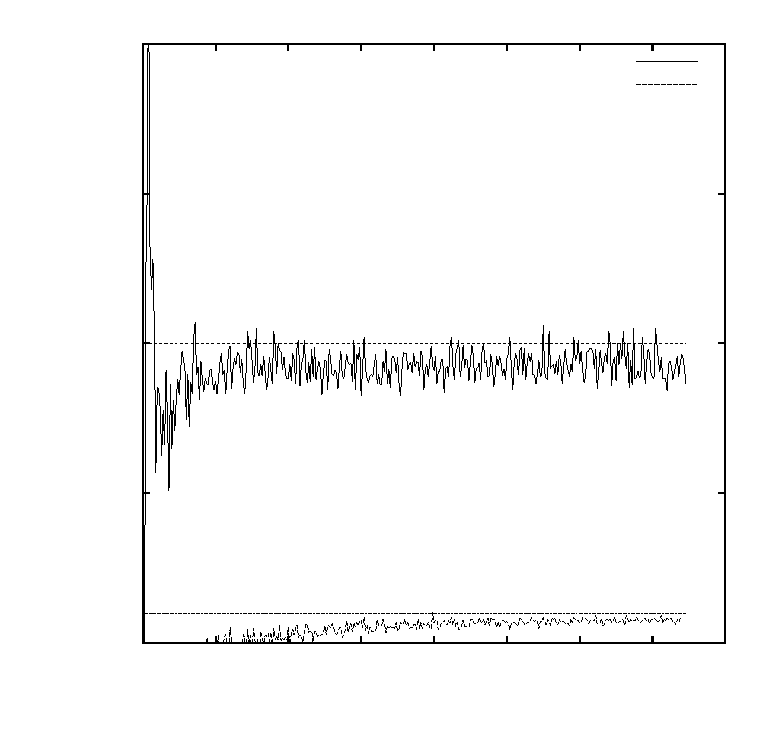
\includegraphics{figures/rho}}%
    \gplfronttext
  \end{picture}%
\endgroup

      \end{tabular}
    }
  \end{center}
\caption{Testing the accuracy of \ty{mlRho}. \textbf{A}: The mutation
  rate estimator, $\hat\theta$, as a function of the sequencing error
  rate, $\epsilon$; sequence length: $10^8$. \textbf{B}: The
  recombination rate estimator, $\hat\rho$, as a function of pairwise
  distance; the data set consists of 1000 pairs of 100kb sequences
  with $\theta=0.01$ and $\epsilon=10^{-4}$; horizontal lines:
  expected value. Coverage: 10.}\label{fig:test}
\end{figure}



\section{Experiments on XSEDE}{\label{sec:experiments}
Migrating from the local cluster Quarry and Mason to Ranger on Xsede is smooth because of the similar computational environment on these clusters. All the data files were easily transferred by standard means. The necessary modules and libraries are all available on Ranger and Stampede.
 
My experience with running mlRho analysis using Bigjob on Ranger consisted of two different phases in terms of the program performance. When we were developing this idea to use Bigjob to run the analysis in an embrassingly parallel way (prior to July 2012), the performance of Bigjob was excellent. All the multicore jobs were completed nicely. However, after the approval of our allocation in September 2012, Bigjob had been upgraded. There seems a number of issues with Bigjob. First of all, the way Bigjob is run involves using the command nohup. As all the jobs are submitted on the login node of Ranger, it is required that no more than 4 nohup commands can be run at one time. It occurred a couple times that I submitted more than 4 bigjobs on the login node and my jobs were all suspended. Subsequently, I was banned from running the jobs. Unfortunately, I was not notified until I found all my jobs were not running for two to three days. This seems to me rather counter productive. For my project, I need to submit ~100 multicore jobs (requiring on average 1024-4096 cores) in total. I would like to have the capacity to submit a number of jobs in the queue and collect data when the jobs are done. Assuming each job is done right, submitting four jobs at a time is not problematic. What is truly problematic is that I encountered a situation that many cores (up to 60\% of the cores) in the same job cannot finish the analysis properly, resulting many missing values. Finding out the missing values and creating new jobs will not necessarily solve the problem, because I often had cores not working properly in these new jobs.
 
We have tried many ways to solve this issue. We thought this might be an issue of our program. Then we implemented the revised code. We used different settings for the Bigjob script. However, none of those helped improve the situation.

The job size was determined based on the scaling test done when preparing our allocation request. Assuming each core can finish simulation for a certain distance with respect to a particular genome size, the number of cores is determined by the total distance for simulation and single job distance.
 
The queuing time on Ranger was largely determined by how many jobs each user have used in the recent past. For a heavy user in the last one or two days, the queuing time might be 1-2 days for new jobs. The Stampede is excellent in terms of queuing time. At this moment, any job gets started almost immediately.

%note from Sen
The speeding up of mlRho program greatly enabled the expansion of this project. Instead of performing analysis to 100 kilo basepairs, we now can carry analyses up to 1 million basepairs.
In fact, the originally proposed work load has been completed. We basically did 10 times more than what we planed to do.

\section{Findings and Preliminary Science Results}\label{sec:results}

\section{Conclusions}\label{sec:conclusion}



%ACKNOWLEDGMENTS are optional
\section{Acknowledgments}
%
% The following two commands are all you need in the
% initial runs of your .tex file to
% produce the bibliography for the citations in your paper.
\bibliographystyle{abbrvnat}
\bibliography{xsede13,references}  % sigproc.bib is the name of the Bibliography in this case
% You must have a proper ".bib" file
%  and remember to run:
% latex bibtex latex latex
% to resolve all references
%
% ACM needs 'a single self-contained file'!
%
%APPENDICES are optional
%\balancecolumns
\end{document}
